\documentclass[a4paper]{article}
\usepackage[pdftex]{graphicx}
\usepackage[utf8]{inputenc}
\usepackage{enumerate}
\usepackage{amssymb}
\usepackage{icomma}
\usepackage{siunitx}
\sisetup{locale=DE} 
\usepackage{tikz}
\usepackage{href-ul}
\hypersetup{
	colorlinks=true,
	linkcolor=blue,
	urlcolor=blue}
\usepackage{geometry}
\geometry{a4paper, top=15mm, left=15mm, right=15mm, bottom=15mm,
	headsep=10mm, footskip=12mm}

\begin{document}
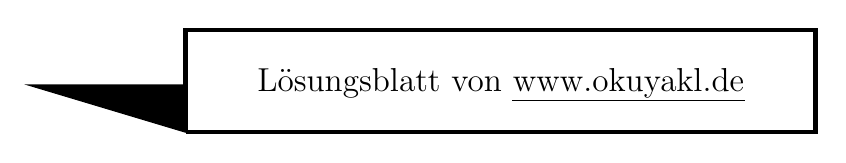
\begin{tikzpicture}(10,3)
	\draw[ultra thick](2,0) --(10,0) -- (10,1.3) --(2,1.3) -- (2,0);
	\draw[fill=black](2,0)-- (0,.6) -- (2,.6) -- (2,0);
	\node at (6,.6) {\large Lösungsblatt von \href{https://www.okuyakl.de}{www.okuyakl.de}};
\end{tikzpicture}
\vspace{0.5 cm}

\noindent{\bf Aufgabe 1. a)}\\
Aus dem Energieansatz $E_{pot}=E_{kin}$ folgt für die Geschwindigkeit der Kugel
im Punkt $B$:
$$v_x=\sqrt{2gy}=\sqrt{2\cdot \SI{9,81}{\meter\over{\second^2}}}\cdot \SI{1,0}{\meter}=\SI{4,4}{\meter\over\second}$$
Dies ist dann auch die Horizontalgeschwindigkeit.
Die Falldauer $t$ erhalten wir mit:
$$
\renewcommand{\arraystretch}{2}
\begin{array}{rcll}

y&=&{1\over 2}gt^2  \\
t&=& \sqrt{2y\over g} \\
t&=& \sqrt{2\cdot \SI{1,0}{\meter} \over \SI{9,81}{\meter\over{\second^2}}} & = \SI{0,45}{\second}
\end{array}
$$
Die Wurfweite $x$ ist dann:

$$x=v_x \cdot t = \SI{4,4}{\meter\over\second}\cdot \SI{0,45}{\second} = \SI{2,0}{\meter}$$

\noindent{\bf Aufgabe 1. b)}\\
Allgemein gilt dann:
$$x(y)=v_x \cdot t =\sqrt{2gy}\cdot  \sqrt{2y\over g} = \sqrt{4gy^2\over g}= 2y$$
Die Wurfweite entspricht also immer genau der Höhe 2y. 
\vspace{0.5 cm}

\noindent{\bf Aufgabe 1. c)}\\
Die Wurfweite ist auf dem Mond genau gleich, da sie unabhängig von $g$ ist.
\vspace{0.5 cm}

\noindent{\bf Aufgabe 2.}\\
Die Horizontalgeschwindigkeit ist $v_x=\SI{50}{\meter\over \second}$
Die Fallzeit ist:
$$t= \sqrt{2h\over g}=\SI{6,4}{\second}$$
Damit ist die Abwurfentfernung:
$$x=v_x\cdot t = \SI{50}{\meter\over \second}\cdot \SI{6,4}{\second} = \SI{320}{\meter}$$
\vspace{0.5 cm}

\noindent{\bf Aufgabe 3.}\\
Die Fallzeit ist:
$$t= \sqrt{2h\over g}=\sqrt{2\cdot \SI{0,020}{\meter}\over \SI{9,81}{\meter\over {\second^2}}}=\SI{0,064}{\second}$$
Damit war die Schussdistanz:
$$x=v_x\cdot t = \SI{310}{\meter}\cdot\SI{0,064}{\second}=\SI{20}{\meter}$$
\vspace{0.5 cm}

\noindent{\bf Aufgabe 4. a)}\\
Horizontalentfernung: 
$$x=\SI{0,134}{\meter}-{1\over 2}\cdot \SI{0,043}{\meter}=\SI{0,113}{\meter}$$
Vertikale Fallstrecke:
$$y={1\over 2}\cdot \SI{0,043} = \SI{0,022}{\meter}$$
\vspace{0.5 cm}

\noindent{\bf Aufgabe 4. b)}\\
Dies entspricht einer Fallzeit von:
$$t=\sqrt{2y\over g}= \SI{0,067}{\second}$$
Für die Horizontalgeschwindigkeit $v_x$ folgt:
$$v_x={x\over t}={\SI{0,113}{\meter}\over \SI{0,067}{\second}}=\SI{1,7}{\meter\over \second}$$
\vspace{0.5 cm}

\noindent{\bf Aufgabe 5.}\\
Die im Flug zu überwindende Horizontaldistanz ist:
$$x=\SI{2,0}{\meter}+{\SI{14}{\meter}\over \tan{\SI{75}{\degree}}} =\SI{5,8}{\meter} $$
Die Fallzeit ist:
$$t=\sqrt{2h\over g}=\sqrt{2\cdot \SI{14}{\meter}\over \SI{9,81}{\meter\over {\second^2}}}=\SI{1,7}{\second}$$
Daraus folgt für die Horizontalgeschwindigkeit:
$$v_x={x\over t}={\SI{5,8}{\meter}\over \SI{1,7}{\second}}=\SI{3,4}{\meter\over \second}$$

\begin{center}
	\includegraphics[width=7 cm]{../../viecher/endcomic.pdf}
	
	Hier geht es zurück zum \href{https://www.okuyakl.de/phys/p9wawL074/aa074.pdf}{Aufgabenblatt}
\end{center}

\end{document}

